\documentclass{article} % For LaTeX2e
\usepackage{iclr2016_workshop,times}
\usepackage{hyperref}
\usepackage{url}

\usepackage[T1]{fontenc}
\usepackage[latin1]{inputenc}
\usepackage{amssymb}
\usepackage{amsmath}
%\usepackage{amsthm}
\usepackage{amsfonts}
\usepackage{graphicx}
%\usepackage[boxed,noend]{algorithm2e}

%\usepackage[algo2e,noend,linesnumbered,boxed]{algorithm2e}
\usepackage[algo2e,noend,boxed]{algorithm2e}
\usepackage{algorithmic}
\usepackage{algorithm}

\usepackage{xspace}
\usepackage{dsfont}
%\usepackage{fullpage}
\usepackage{graphicx}  
\usepackage{verbatim}
\usepackage{appendix}
\usepackage{multirow}
\usepackage{color}
\usepackage{framed}
\usepackage{wrapfig}
\newtheorem{thm}{Theorem}%[section]
\newtheorem{cor}[thm]{Corollary}
\newtheorem{lem}[thm]{Lemma}
\newtheorem{prop}[thm]{Proposition}
\newtheorem{prob}[thm]{Problem}
\newtheorem{example}[thm]{Example}
%\theoremstyle{definition}
%\newtheorem{defn}[thm]{Definition}
%\theoremstyle{remark}
%\newtheorem{rem}[thm]{Remark}

%\newcommand{\shadecolor}{white}
\definecolor{shadecolor}{rgb}{.6,.6,.6}
\newenvironment{highlight}[1][gray]%
 {\vspace*{0.5\baselineskip}
\begin{center}\begin{minipage}{0.85\textwidth}\begin{shaded}}%
 {\end{shaded}\end{minipage}\end{center} \vspace*{0.5\baselineskip}}

% enable subfigures
\usepackage[tight,scriptsize]{subfigure}
%\usepackage{subfloat}
\newcommand{\denselist}{
\itemsep -2pt\topsep-8pt\partopsep-8pt
}
\newcommand{\loud}[1]{\textcolor{green}{!!!! #1 !!!!}}

\newcommand{\Jon}[1]{{\color{red}{\bf\sf [Jon: #1]}}}
\newcommand{\Kevin}[1]{{\color{blue}{\bf\sf [Jon: #1]}}}
\newcommand{\kevin}[1]{{\color{blue}{\bf\sf [Jon: #1]}}}

\vfuzz2pt % Don't report over-full v-boxes if over-edge is small
\hfuzz2pt % Don't report over-full h-boxes if over-edge is smallq
\numberwithin{equation}{section}
\newcommand{\abs}[1]{\lvert#1\rvert}
\newcommand{\blankbox}[2]{%
  \parbox{\columnwidth}{\centering
    \setlength{\fboxsep}{0pt}%
    \fbox{\raisebox{0pt}[#2]{\hspace{#1}}}%
  }%
}
\newcommand{\blockcomment}[1]{ }

\newcommand{\tr}{\mbox{Tr }}
\newcommand{\bfi}{\bfseries\itshape}
\def\reals{\mathbb{R}}
\def\rationals{\mathbb{Q}}
\def\borel{\mathbb{B}}
\newcommand{\complex}{\mathbb{C}}
\newcommand{\eqbase}{1/2}
\newcommand{\eqalt}{\sqrt{3}/2}
\newcommand{\im}{\mbox{im }}
\def\naturals{\mathbb{N}}
\def\expectation{\mathbb{E}}
\def\normal{\mathcal{N}}
\def\Tr{\mbox{Tr}}
\def\triv{{\bf 1}}

\newcommand{\drho}[1]{d_{\rho_{#1}}}
\newcommand{\twovec}[2]{\left[
\begin{array}{c}
#1 \\
#2 \\
\end{array}\right]
}
\newcommand{\twomat}[4]{\left[
\begin{array}{cc}
#1 & #2 \\
#3 & #4 \\
\end{array}\right]
}
\newcommand{\threemat}[9]{\left[
\begin{array}{ccc}
#1 & #2 & #3 \\
#4 & #5 & #6 \\
#7 & #8 & #9 \\
\end{array}
\right]
}
\newcommand{\threematbl}[4]{\left[
\begin{array}{cccc}
1 & \vline & 0 & 0 \\
\hline
0 & \vline & #1 & #2 \\
0 & \vline & #3 & #4 \\
\end{array}
\right]
}
\def\triv{{\bf 1}}
\def\post{\widehat{L^{(t)}P^{(t)}}}
\def\postbra{\left[\post\right]}
\newcommand{\Conditioning}{{\sc KroneckerConditioning} \xspace}
\newcommand{\PredictionRollup}{{\sc PredictionRollup} \xspace}
\newcommand{\ComputeCG}{{\sc ClebschGordanCoeffs} \xspace}
\newcommand{\ind}[1]{\mathds{1}\left\{#1\right\}}
\newcommand{\algref}[1]{Algorithm~\ref{#1}}
\newcommand{\invFourier}[3]{
\hat{#1}_{\rho_{#3}}^T \cdot #2_{#3}(\sigma)
}

\newbox\subfigbox
\makeatletter
\newenvironment{subfloat}
{\def\caption##1{\gdef\subcapsave{\relax##1}}%
\let\subcapsave\@empty\setbox\subfigbox\hbox
\bgroup}{\egroup\subfigure[\subcapsave]{\box\subfigbox}}
\makeatother

\newcommand\T{\rule{0pt}{3.7ex}} %top strut
\newcommand\B{\rule[-3.1ex]{0pt}{0pt}} %bottom strut
\newcommand\TT{\rule{0pt}{2.7ex}} %top strut
\newcommand\BB{\rule[-1.8ex]{0pt}{0pt}} %bottom strut



\include{wrapfig}
%\title{Interpretable deep layered models for generating images with   occlusion}
%\title{Learning to invert deep layered image models using inference networks}
\title{Efficient inference in occlusion-aware generative models of images}

\author{Jonathan Huang \& Kevin Murphy \\
Google Research \\
1600 Amphitheatre Parkway \\
Mountain View, CA 94043, USA\\
\texttt{\{jonathanhuang, kpmurphy\}@google.com}
}


\newcommand{\fix}{\marginpar{FIX}}
\newcommand{\new}{\marginpar{NEW}}


%\iclrfinalcopy % Uncomment for camera-ready version

\begin{document}


\maketitle

\begin{abstract}
We present a generative model of images based on layering,
in which image layers are individually generated, then composited
from  front to back.  We are thus able to factor the appearance
of an image into the appearance of individual objects within the image --- and additionally for
each individual object, we can factor content from pose.  
Unlike prior work on layered models, we learn a shape prior for each
object/layer, allowing 
the model to tease out which object is in front by looking for a consistent shape,
without needing access to motion cues
or any labeled data.
We show that ordinary stochastic gradient variational bayes (SGVB), which optimizes our fully differentiable
lower-bound on the log-likelihood, is sufficient to learn an interpretable representation of images.
Finally we present experiments demonstrating the effectiveness of the model for inferring foreground
and background objects in images.
\end{abstract}


\section{Introduction}


Recently computer vision has made great progress by training deep
feedforward neural networks on large labeled datasets.
However, acquiring labeled training data for all of the problems that
we care about is expensive.
Furthermore, some problems require top-down inference as well as
bottom-up inference in order to handle ambiguity.
For example, consider the problem of object detection
and instance segmentation  in the
presence of clutter/occlusion.,
 as illustrated in Figure~\ref{fig:cows}.
In this case, the foreground object may
obscure almost all of the background object, yet people are still able
to detect that there are two objects present, to correctly segment
out both of them, and even to amodally complete the hidden parts of
the occluded object (cf., \cite{Kar2015}).


\begin{wrapfigure}[11]{r}[12pt]{6cm}
\vspace{-4mm}
\begin{center}
    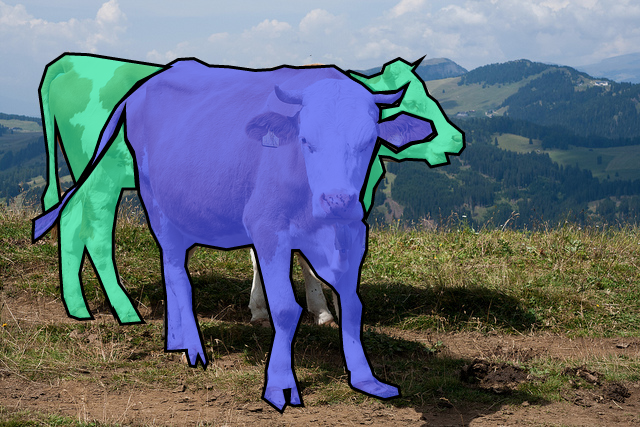
\includegraphics[width=0.375\textwidth]{figs/two_cows.png} \vspace{-2mm}
    \caption{\footnotesize Illustration of occlusion.}
    \label{fig:cows}
  \end{center}
  \vspace{-2mm}
\end{wrapfigure}



One way to tackle this problem is to use generative models.
In particular, we can imagine the following generative process for an image:
(1) Choose an object (or texture) of interest, by sampling a ``content vector''
representing its class label, style, etc;
(2) Choose where to
place the object in the 2d image plane, by sampling a ``pose vector'',
representing location, scale, etc. 
(3) Render an image of the object onto a hidden canvas or layer;\footnote{
We  use  ``layer''  in this paper mainly to refer to image layers, however
in the evaluation section (Section~\ref{sec:eval}) ``layer'' will also be used to refer to
neural network layers where the meaning will be clear from context.
}
(4) Repeat this process for $N$
objects (we assume in this work that $N$ is fixed);
(5) Finally, generate
the observed image by compositing the layers in order.\footnote{
%
There are many  ways to composite multiple layers in computer
graphics~\citep{porter1984compositing}. 
In our experiments, we use  the classic \emph{over operator}, which
reduces to a simple $\alpha$-weighted 
convex combination of foreground and background pixels,
in the two-layer setting.
 See Section~\ref{sec:models} for more details.
}

\looseness -1 There have been several previous attempts to use layered generative
models to perform scene parsing and object detection in clutter (see
Section~\ref{sec:related} for a review of related work). However, such
methods usually run into computational bottlenecks, since inverting
such generative models is intractable.
In this paper, we build on recent work (primarily \cite{Kingma2014,gregor2015draw})
that shows how to jointly train a generative model and an inference
network in a way that optimizes a variational lower bound on the log
likelihood of the data;
this has been called a ``variational auto-encoder'' or VAE.
In particular, we extend this prior work in
two ways. First, we extend it to the sequential setting, where we
generate the observed image in stages by compositing hidden layers
from front to back. %back to front. 
Second, we combine the VAE with the spatial transformer network of
\citep{jaderberg2015spatial}, allowing us to factor out variations
in pose (e.g., location) from variations in content (e.g., identity).
We call our model the ``composited spatially transformed VAE'', or CST-VAE
for short.

Our resulting inference algorithm combines top-down (generative)
and bottom-up (discriminative) components in an interleaved fashion as follows:
(1)  First we recognize (bottom-up) the foreground object, factoring apart pose and content;
(2) Having recognized it, we generate (top-down) what the hidden image  should look
like;
(3) Finally, we virtually remove this generated hidden image from the observed
image to get the residual image, and we repeat the process.
(This is somewhat reminiscent of approaches that the brain is believed
to use, \cite{Hochstein2002}.)

The end result is a way to factor an observed image of
overlapping objects into $N$
hidden layers, where each layer contains a single object
with its pose parameters.
Remarkably, this whole process can be trained in a fully unsupervised
way using standard gradient-based optimization methods
(see Section~\ref{sec:models} for details).
In Section~\ref{sec:eval}, we show that our method is able to reliably
interpret cluttered images, and that the inferred latent
representation is a much better  feature vector for a discriminative
classification task than working with the original cluttered images.

\vspace{-3mm}


\eat{
Large strides have been made in computer vision in recent years 
due to scalable deep learning and massive labeled datasets such as Imagenet~\cite{krizhevsky2012imagenet,deng2009imagenet}.
But as we move beyond simple image classification problems to more complication output spaces, the limitations
to our current approaches are becoming more transparent.
Dense labeling problems such as semantic segmentation, instance segmentation, for example,
require much more human effort per image to label and more images in general.




We've seen less progress on unsupervised models  ---  using MCMC

traditional graphical models from yesteryear (citations?) 	- methods tend to be less scalable often requiring intractable normalization constants to be computed
  --- recent work has bypassed this (citations) allowing models to be trained via gradient methods


Things don't just have one label

We also are starting to get interested in dense labels of images and video: think semantic segmentations, instance level segmentations, depth, etc.
	It's getting more and more expensive to collect this data.

	
Unsupervised and weakly supervised models are the next frontier.  

The goal is to model the variation in real images.  
Disentangling the factors of variation is critical to confronting the curse of dimensionality.

conv nets for example learn higher levels of abstraction, disentangling variation in appearance

there has been some work in the deep learning community factoring pose from appearance.

No work on factoring out the variability stemming from Multiple objects.

We propose a layered model of image generation.  And it has these benefits.


\Jon{play up interpretability of the model}


A critical issue in counting and instance level segmentation is dealing with things that can overlap and partially occlude each other, and current detection methods that use non-max suppression, for example, are not smart at reasoning about overlap/occlusion.  

In the instance segmentation problem, for example, we might need to analyze a local patch and decide whether it belongs to instance A, or instance B, or whether there were even two instances that were overlapping to begin with.  In some of these settings, the decision cannot be made at the local level and requires a global understanding of the semantics of the scene.


Motivations:
	The idea that we explore here is: if we only knew what the instances A and B were supposed to look like (i.e., had pixel-level generative models of A and B), we would be better positioned to make this decision.

	Being able to do this can help in a ton of applications: counting, instance segmentation
		even training for object recognition ? a lot of examples are occluded and if knew how
			how to factor out this variation, it could help
			
	But we can go further: we can imagine what?s behind (amodal completion)

	A step toward integrating top-down and bottom-up
	
	part of the story is that we're able to use VAEs to now combine some of the prior structure that we know about 
		with the rich expressiveness of deep models and train them all together with backprop

We propose a generative model that separately generates a ?layer? for each object in the image
in which each layer itself we?ve separated pose from style.
\begin{itemize}
\item fully unsupervised training (?) using ordinary sgd based methods that use backprop
\item st-aevb model
\item new ?alpha compositing? layer which is kind of like a pixelwise attention mechanism
\item masked inference mechanism allowing for training from partially observed images
\item usage of conv and deconv layers in a fully probabilistic generative model
\item show how to reason with occlusions and do amodal completion of objects based on a generative model
can handle multiple and unknown number of objects?
\end{itemize}
}

\section{Related work}
\label{sec:related}
\vspace{-2mm}

\subsection{Deep probabilistic generative models}
\vspace{-2mm}
Our approach is inspired by the recent introduction of generative deep learning models that can be
trained end-to-end using backpropagation.  These models have included
generative adversarial networks \citep{denton2015deep, goodfellow2014generative}
as well as variational auto-encoder (VAE) models \citep{Kingma2014,kingma2014semi,rezende2014stochastic,burda2015importance}
which are most relevant to our setting.  

Among the variational auto-encoder works, our work is most comparable to 
the DRAW network of~\cite{gregor2015draw}.  As with our proposed model, 
the DRAW network is generative model of images in the variational auto-encoder framework
that decomposes image formation into multiple stages of additions to a canvas matrix.  
Where their paper assumes a generic LSTM based generative model of these sequential 
drawing actions, however, we enforce a prior that allows our stages to have an intuitive interpretation
as layers (that one might use in typical photo editing software).


%VAE papers
%		importance weighted auto-encoders \cite{burda2015importance}
%		 VAE papers \cite{Kingma2014, kingma2014semi,rezende2014stochastic}
%		DRAW \cite{gregor2015draw}
%		Tejas Kulkarni?s paper \cite{kulkarni2015deep}	
%		Adversarial networks \cite{denton2015deep, goodfellow2014generative}
		
%These papers are deep (and sort of generative) but definitely not probabilistic
%Texture generation \cite{gatys2015a, gatys2015b}
	
%\Jon{We specifically need to spend some time differentiating from the DRAW network
%	which is by far the most related to the final proposed model.  The biggest difference is the RNN
%	which assumes that layers (what they call glimpses) are dependent on past layers (both in the 
%	generative model as well as in the recognition model.
%	 Other differences: they use an attention model which seems to help a lot --- our spatial
%	 transformer part can also be interpreted as a kind of attention model (but it's not really the same).
%	 They also composite using a different (less interpretable) function.
%	}
\vspace{-2mm}
\subsection{Modeling Transformation in neural networks}\vspace{-2mm}
One of our major contributions is a model that is capable of separating the pose of an object from its appearance,
which is of course a classic problem in computer vision \Jon{is there a really ancient paper that we can cite here? The older the better }. 
Here we highlight several of the most related works from 
the deep learning community.  
Many of these work related works have been influenced by \cite{hinton2011transforming} on Transformed Auto-encoder models,
in which pose is explicitly separated from content in an autoencoder which is trained to predict (known)
small transformations of an image 
More recently,  \cite{dosovitskiy2014learning} introduced a convolutional network to generate images of chairs where pose was explicitly separated out, and \cite{cheung2014discovering} introduced an auto-encoder where a subset of variables such as pose can be explicitly observed and remaining
variables are encouraged to explain orthogonal factors of variation.   
Most relevant in this line of works is that of~\cite{kulkarni2015deep}, which, like us, 
separate the content of an image from pose parameters using a variational auto-encoder.
In all of these works, however, there is an element of supervision, where variables such as pose
and lighting are known at training time. 
%To achieve this separation, however, they train 
%rely on a custom training procedure in whic.
Our method in contrast is able to separate pose from content in an fully unsupervised setting 
using standard off-the-shelf minibatch gradient methods.




Finally our method relies crucially on the recently introduced Spatial
Transformer Networks paper
 ~\citep{jaderberg2015spatial}, which introduced 
a fully differentiable module that allows one to warp/rotate images based on some input spatial transformation.
To our knowledge, we are the first to apply this module in an unsupervised learning setting.  

%	Discovering Hidden Factors of Variation in Deep Networks \cite{cheung2014discovering},
%	Chair paper \cite{dosovitskiy2014learning}: The above two papers both separate style from pose (and other things like lighting) but use ordinary autoencoders which do not have the same probabilistic semantics.  They also train their models in a supervised setting and thus required labeled data for pose/lighting/etc
\vspace{-2mm}
\subsection{Layered models and amodal completion}\vspace{-2mm}
Layer based models have been used in a number of works in computer vision  --- traditionally
taking advantage of motion cues to decompose video data into layers~\citep{wang1994representing,ayer1995layered,kannan2005generative}.
However there have been works that apply layer based reasoning on images.
\cite{yang2012layered}, for example, propose a layered model for
segmentation but rely heavily on bounding box and categorical
annotations.	
\cite{Isola2013} deconstruct a single image into layers, but require a
training set of manually segmented regions.
Our model also has similarities to that of \cite{le2011learning}, however  they use restricted Boltzmann machines, 
which require expensive MCMC sampling to estimate gradients and have difficulties reliably estimating the 
log-partition function.  %ur model¯
%falls under the category of variational autoencoders which do not require expensive MCMC sampling.	
	
%Amodal completion, where one must ``complete'' a partially visible object, is a challenging vision task
%that several papers have recently attempted.
% has recently been a
%Though we do not attempt the amodal completion task on a large scale vision dataset,
%we believe that generative models such as the one we propose could potentially be very useful in this task.
%\cite{amodalKarTCM15}, \cite{categoryShapesKar15}, \cite{zhu2015semantic}
	
	


% all use motion cues to decompose a video into layers
%	The kannan model (at least the graphical model part) looks a lot like ours except they 
%		treat videos and rely on motion cues.  They don't assume that appearance is encoded from some latent vector ---
%		rather they treat appearance as a pixel matrix which can be warped by motion throughout the video	
%	They use EM with variational inference
	
	
	
		
	
	
	
	
	
	
	


\section{CST-VAE: A probabilistic layered model of image generation}
\label{sec:models}\vspace{-3mm}




%In this section we build up to our 
%main contribution, the Composited Spatially Transformed Variational Auto-encoder model in three pieces. 
%We first review the (vanilla) Variational Auto-encoder model, a deep generative model that
%was recently proposed  in~\cite{Kingma2014}.  We next show how to factor pose from content
%by introducing Spatially Transformed Variational Auto-encoders (ST-VAE).  Compositing multiple image layers generated
%by ST-VAE modules 
%finally allows us to create our desired CST-VAE model.


\begin{figure}[t]
\begin{center}
\subfigure[]{
\raisebox{1mm}{
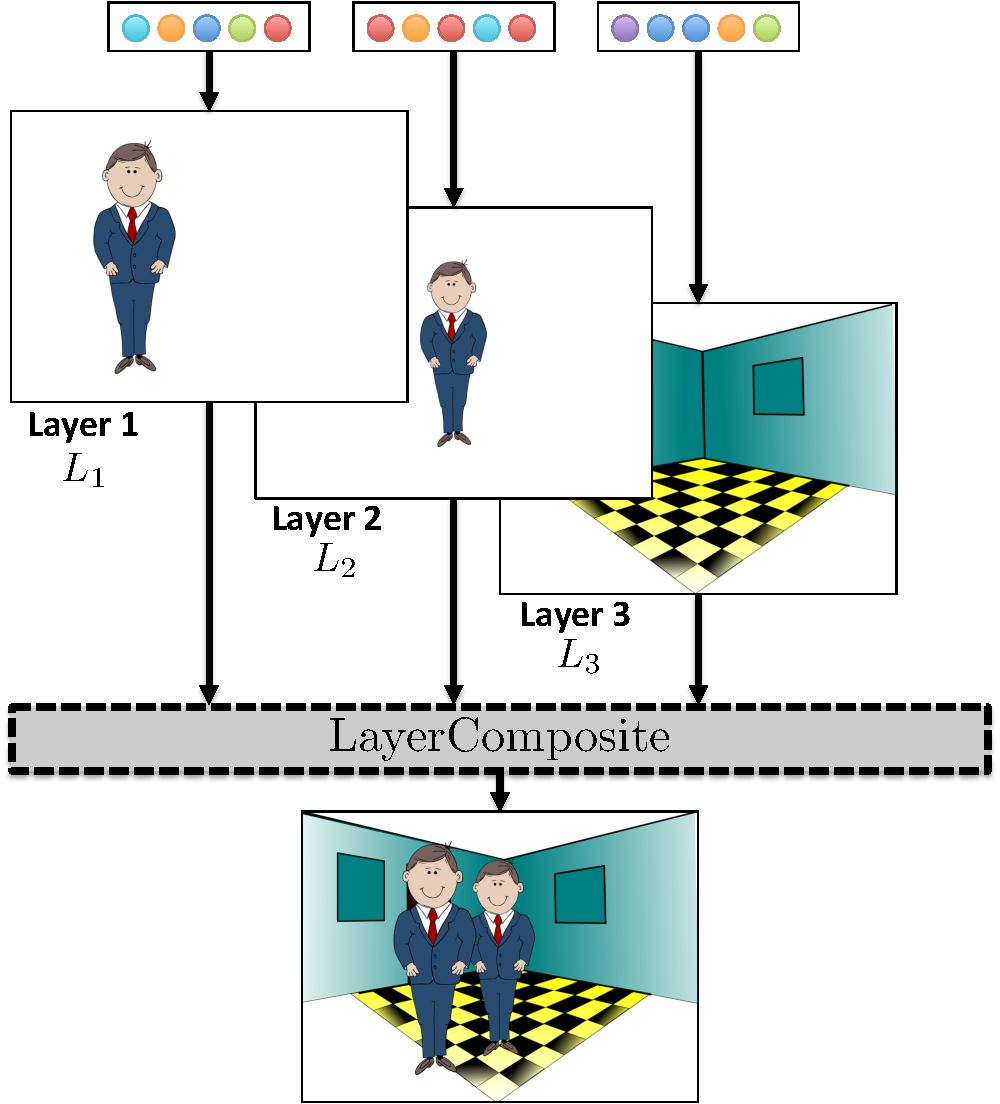
\includegraphics[width=0.30\linewidth]{figs/cartoon.pdf}
\label{fig:cartoon}
}
}\qquad\qquad\qquad
\subfigure[]{
%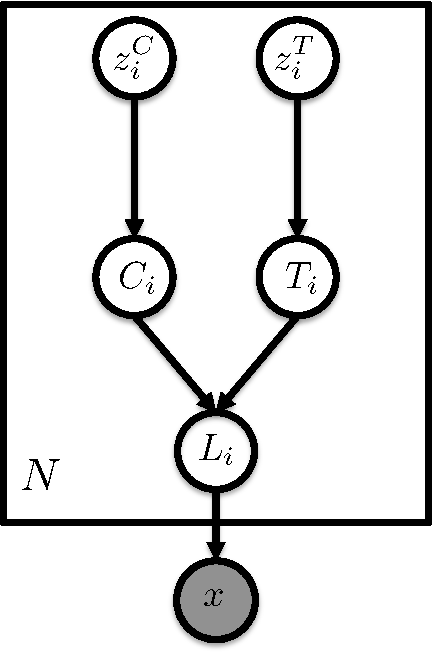
\includegraphics[width=0.2\linewidth]{figs/compositestvae_graphicalmodel.pdf}
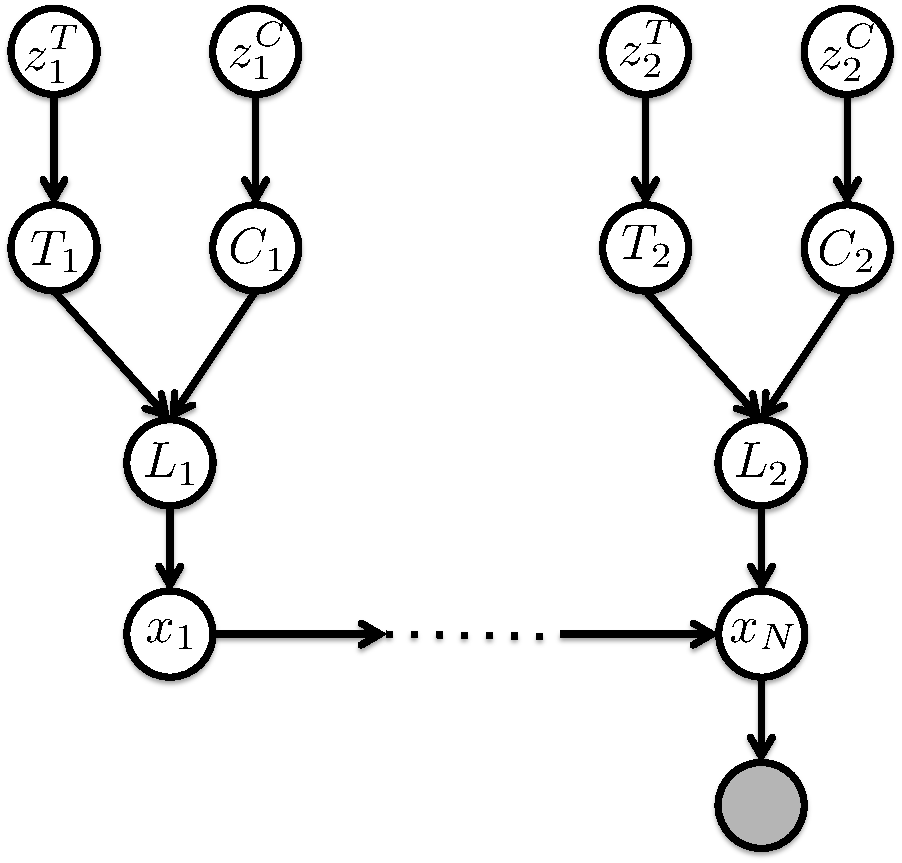
\includegraphics[width=0.35\linewidth]{figs/cstVae2.pdf}
\label{fig:compositestvae_gm}
}\vspace{-3mm}
\end{center}
 \caption{\footnotesize \subref{fig:cartoon} Simplified cartoon illustration of the CST-VAE layer compositing process; 
 \subref{fig:compositestvae_gm} CST-VAE graphical model.  
%The boxed  portion of the graph (plate notation) is duplicated $N$ times. 
%\Jon{fix notation here and label the cartoon with variables}.
% Note that the order of the layers matters (to reflect that foreground can occlude background but not vice versa).
 }
\label{fig:stvaemodel}
\end{figure}


In this section we introduce the \emph{Composited Spatially Transformed Variational Auto-encoder  (CST-VAE)},
a family of latent variable models, which factors
the appearance of an image into the appearance of the different layers
that create that image.  
Among other things, the CST-VAE model allows us to tease
apart the component layers (or objects) that make up an image and reason about occlusion in order to perform tasks such as amodal completion or instance segmentation.
Furthermore, it can be trained in a fully unsupervised fashion using  minibatch stochastic
gradient descent methods but can also make use of labels in supervised or semi-supervised settings.
 
 In the CST-VAE model, we assume that images are created by (1) generating a sequence of image layers 
 then (2) compositing the layers to form a final result $x$.  Figure~\ref{fig:cartoon} shows a simplified cartoon illustration of this process.  
 We now discuss these two steps individually.
 \vspace{-1mm}
 \paragraph{Layer generation.}
 The layer generation model is interesting in its own right and we will call it the ST-VAE model (since there is no compositing step).
 We intuitively think of  layers as corresponding to objects in a scene --- a layer $L$ is assumed 
 to be generated by first generating an image $C$ of an object in some canonical pose (we refer to this image as
 the \emph{canonical image} for layer $L$), then warping $C$ in the 2d image plane (via some transformation $T$).
We assume that both $C$ and $T$ are generated by some latent variable --- specifically $C = f_C(z^C; \theta_C)$ and $T = f_T(z^T; \theta_T)$,
where $z^C$ and $z^T$ are latent variables and $f_C(\cdot; \theta_C)$ and $f_T(\cdot; \theta_T)$ are nonlinear functions with parameters
$\theta_C$ and $\theta_T$ to be learned. \Jon{content and pose generators}
We are agnostic as to the particular parameterizations of $f_C$ and $f_T$, though as we discuss below, they
are assumed to be almost-everywhere differentiable and in practice we have used MLPs and convolutional networks.
In the interest of seeking simple interpretations of images, we assume that these latent pose and content ($z$) variables are low 
dimensional and independently Gaussian.

Finally to obtain the warped image, we
use \emph{Spatial Transformer Network} (STN) modules, recently introduced by~\cite{jaderberg2015spatial}.
We will denote  the result of resampling an image $C$ onto a regular grid which has been transformed by $T$ by $STN(C, T)$.
The benefit of using STN modules in our setting 
is that they perform resampling in a differentiable way, allowing for our models to be trained using gradient methods.
 \vspace{-1mm}
\paragraph{Compositing.}
To form the final observed image of the CST-VAE model, we generate a sequence of layers $L_1$, $L_2$, \dots, $L_N$
independently drawn from the ST-VAE model and composite from front to back.
There are many  ways to composite multiple layers in computer graphics~\citep{porter1984compositing}.
In our experiments, we use  the classic \emph{over operator}, which reduces to a simple $\alpha$-weighted
convex combination of foreground and background pixels (denoted as a  binary  operation $\oplus$)
in the two-layer setting, but can be iteratively applied
to handle multiple layers. % associativity of the over operator

 

To summarize, the CST-VAE model can be written as the following generative process.  Let $x_0=\mathbf{0}^{w\times h}$ (i.e., a black image).   For $i=1,\dots,N$:\vspace{-4mm}

{\footnotesize
\begin{align*}
z_i^C, z_i^T  &\sim \mathcal{N}(0, I), \\
C_i &= f_C(z_i^C; \theta_C), \\
T_i &= f_T(z_i^T; \theta_T), \\
L_i &= \mbox{STN}(C_i, T_i), \\
x_i &= x_{i-1} \oplus L_i.
\end{align*}\vspace{-4mm}
}

The final image pixels are then drawn conditioned on the pixels of $x_N$.  For binary images,
setting the last $x_i$ as the observed image (i.e., $x\equiv x_N$). \Jon{not quite right yet ---
if images are binary, then we model $P(x| x_N)$ as a bernoulli.  If it's continuous, then $P(x|x_N)$ could be Gaussian.}
See Figure~\ref{fig:compositestvae_gm} for
 a graphical model depiction of the CST-VAE generative model.




\subsection{Inference and parameter learning with variational auto-encoders}

In the context of the CST-VAE model, we are  interested in two coupled problems:
``explaining'' an observed image $x$ by inferring all of the latent variables $z^C_i$ and $z^T_i$ given the model parameters $\theta$  (\textbf{inference}), and 
 estimating the model parameters $\theta=\{\theta_C,\theta_T\}$ given a training set of images $\{x^{(i)}\}_{i=1}^m$ (\textbf{learning}).  
Traditionally for  latent variable models such as CST-VAE,  one might solve these problems using EM~\citep{dempster1977maximum}
with approximate inference (e.g., loopy belief propagation, MCMC or mean-field) ~\citep{wainwright2008graphical}. 
However if we want to allow for rich expressive parameterizations of the generative models $f_C$ and $f_T$, the integrals required
for these approximate inference approaches become intractable.  Instead we use the recently proposed 
variational auto-encoder (\emph{VAE}) framework~\citep{Kingma2014} for inference and learning.

In the variational auto-encoder setting, we assume that the posterior distribution over latents is parameterized by a particular form
 $Q(z^C, z^T|x;\phi)$ and the goal is to find a setting of
the parameter $\phi$ to make $Q$ (called a \emph{recognition model}) a good approximation to the posterior.  
In contrast to typical mean-field approximations for latent variable models,
we learn a single setting for $\phi$ rather than optimizing variational parameters for each example. 
Specifically we optimize the following expression
jointly with respect to generative model parameters $\theta$ and recognition model parameters $\phi$:
\begin{equation}\label{eqn:vae_objective}\footnotesize
\mathcal{L}(\theta, \phi; \{x^{(i)}\}_{i=1}^m)
	= \sum_{i=1}^m \frac{1}{S}\sum_{s=1}^S \left[-\log Q(z_{i,s}^C, z_{i,s}^T | x^{(i)};\phi) + \log P(x^{(i)} | z_{i,s}^C, z_{i,s}^T; \theta) \right],
\end{equation}
%\expectation_{Q(z_\ell^C, z_\ell^T | x^{(i)};\phi)} 
where $z_{i,s}^C, z_{i,s}^T \sim Q(z^C, z^T | x^{(i)};\phi) $ are samples drawn from the variational posterior $Q$.
%\kevin{use $s$ as an index for samples, since $\ell$ is for
%  layers. Comment that all layers are deterministic except for z and
 % the final x.}

Equation~\ref{eqn:vae_objective} is stochastic lower bound on the observed data log-likelihood and interestingly,
is differentiable with respect to parameters $\theta$ and $\phi$ in certain situations. In particular,
%The posterior parameterization $Q$ is sometimes called a \emph{recognition model} or a probabilistic \emph{encoder} (since we can
%think of the latent variable $z$ as being a code
when $Q$ is Gaussian and the likelihood under the generative model $P(x|z^C,z^T; \theta)$ is differentiable, 
then the stochastic variational lower bound can be written in an end-to-end
differentiable way via the so-called \emph{reparameterization trick} introduced in ~\cite{Kingma2014}.
Furthermore, the objective in Equation~\ref{eqn:vae_objective} can be interpreted as a reconstruction cost plus regularization term on the middle layer
of a neural network, which is why we think of these models as auto-encoders.  
For this reason, the generative model $P(x|z^C, z^T )$ is also called a decoder (more specifically we will
refer to $f_C$ as the content decoder and $f_T$ as the pose decoder) and the recognition model $Q(z^C, z^T|x;\phi)$
is called an encoder.

In the following, we discuss how to do parameter learning and inference for the CST-VAE model
within the variational auto-encoder framework more specifically.
The critical design choice that must be made is how to parameterize  the recognition model $Q$. There are two things 
that we hope for in a recognition model: (1) it must be able to 
capture the important dependencies that may arise in the posterior; (2) we should be able to differentiate the result of
sampling $Q$ with respect to its parameters $\phi$.  The second desiderata is accomplished (as is standard in VAE models)
by parameterizing $Q$ as a normal distribution (whose mean and variance are nonlinear functions of $\phi$), allowing us to differentiate using the 
reparametrization trick.  



%Unfortunately traditional approaches such as EM
%$P(x;\theta) = \int P(x| z^T, z^C) P(z^T) P(z^C)$






%\subsection{{\bf VAE} Model: Variational Auto-encoder}\label{sec:vae}

%Throughout this section, we are concerned with the following latent variable model.
%Given a collection of i.i.d. samples $\{x_i\}_{i=1}^N$, we assume that each sample $x$
%is generated by first drawing a variable $z$ independently from a prior distribution $P_\theta(z)$
%then drawing $x$ conditioned on $z$ from $P_\theta(x|z)$.  %Thus we assume $P_\theta(x) = \int_z P_\theta(x | z) P_\theta(z) dz$.

%The variable $z$ is assumed to be unobservable 
%and we are thus interested in two coupled problems:
%(inference) inferring $z$ given an observation $x$ and model parameters $\theta$, and 
%(learning) estimating the model parameters $\theta$ given a collection of $x$.

%If we want to model complicated data (e.g., images), however, we need to allow for rich conditional distributions
%$P_\theta(x|z)$, which leads to complicated posteriors $P_\theta(z|x)$ making inference and learning intractable.

%In the variational auto-encoding setting, we assumed a fixed form for the posterior distribution $Q_\phi(z|x)$ and optimize
%the parameter $\phi$ to make $Q$ a good approximation to the posterior.  In contrast to typical mean-field approximations for latent variable models,
%this optimization is not done per-instance    
%Specifically we optimize the following 
%which is a lower bound on the observed data log-likelihood:
%\begin{equation}\label{eqn:vae_objective}
%\mathcal{L}(\theta, \phi; x_i)
%\end{equation}


%Both of the models that we discuss later in this section (i.e., ST-VAE and CST-VAE) fall under the category of variational auto-encoders,
%which was 



\subsection{{\bf ST-VAE} Spatially Transformed Variational Auto-encoder}\label{sec:stvae}\vspace{-3mm}
\begin{figure}[t]
\begin{center}
\subfigure[]{
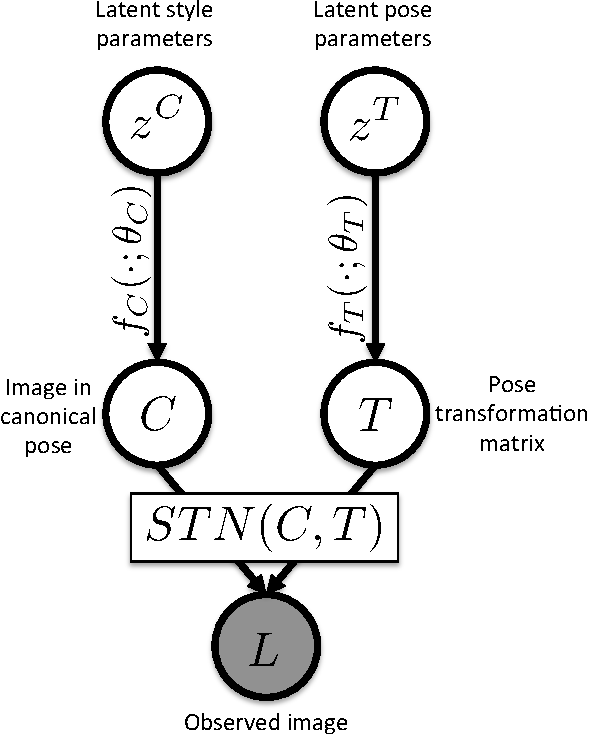
\includegraphics[width=0.25\linewidth]{figs/stvae_gen.pdf}
\label{fig:stvae_decoder}
}\qquad\qquad
\subfigure[]{
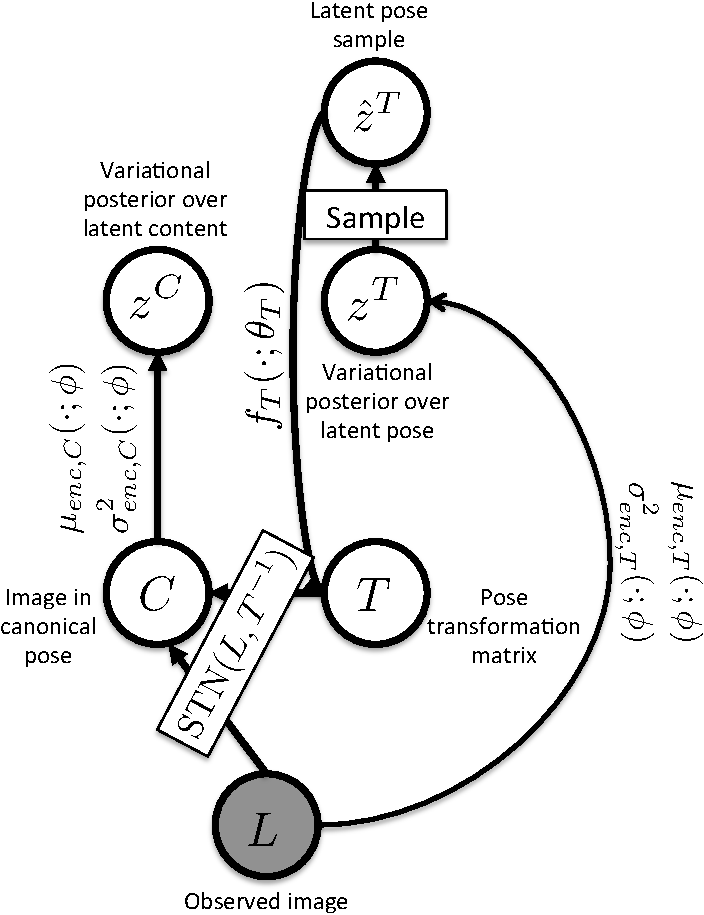
\includegraphics[width=0.3\linewidth]{figs/stvae_rec.pdf}
\label{fig:stvae_encoder}
}\vspace{-4mm}
\end{center}
 \caption{\footnotesize
 \subref{fig:stvae_decoder} ST-VAE Generative model, $P(L | z^C, z^T)$ (Decoder); \subref{fig:stvae_encoder} ST-VAE Recognition model $Q(z^C,z^T | L) = Q(z^C | z^T, L)\cdot Q(z^T | L)$ (Encoder)   
  }\vspace{-5mm}
\label{fig:stvaemodel}
\end{figure}


We focus first on how to parameterize the recognition network (encoder) for the simpler case of a single layer model (i.e., the ST-VAE model
shown in Figure~\ref{fig:stvae_decoder}), in which we need only predict a single set of latent variables $z^C$ and $z^T$.
Na\"{i}vely, one could 
simply use an ordinary MLP to parameterize a distribution $Q(z^C, z^T | L)$, but ideally we would take advantage of the same
 insight that we used for the generative model: that it is advantageous to model content from images of objects in a canonical pose instead
 of conflating content with pose.  To this end, we propose the ST-VAE recognition model shown in Figure~\ref{fig:stvae_encoder}. 
Conceptually the ST-VAE recognition model breaks the prediction of $z^C$ and $z^T$ into two stages.  Given the observed image $L$,
we first predict the latent representation of the pose, $z^T$.  Have this latent $z^T$ allows us to recover the pose transformation 
$T$ itself, which we use to ``undo'' the transformation of the generative process
by using the Spatial Transformer Network again but this time with the inverse transformation of the predicted pose.  This result, which can be
thought of as a prediction of the image in a canonical pose is finally used to predict latent content parameters.


More precisely, we assume that the joint posterior distribution over
pose and content factors as
$Q(z^C, z^T | L) = Q(z^T |L)\cdot Q(z^C | z^T, L)$ where both factors are normal distributions.  
To obtain a draw $(\hat{z}^C, \hat{z}^T)$ from this posterior, we use the following procedure:\vspace{-4mm}

{\footnotesize
\begin{align*}
\hat{z}^T &\sim Q(z^T |L; \phi) = \mathcal{N}(\mu_{T}(L; \phi), \mbox{diag}(\sigma_{T}^2(L; \phi))), \\
\hat{T} &= f_T(\hat{z}^T), \\
\hat{C} &= \mbox{STN}(L, \hat{T}^{-1}), \\
\hat{z}^C &\sim Q(z^C | z^T, L; \phi) =  \mathcal{N}(\mu_{C}(\hat{C}; \phi), \mbox{diag}(\sigma_{C}^2(\hat{C}; \phi))).
\end{align*}\vspace{-2mm}
}
%\kevin{Just write $\mu_{T}()$ instead of $\mu_{enc,T}$. Maybe we need a
%  table summarizing notation?}

To train an ST-VAE model, we then use the above parameterization of $Q$ and maximize Equation~\ref{eqn:vae_objective} with minibatch
SGD.
As long as the pose and content encoders and decoders  are differentiable, Equation~\ref{eqn:vae_objective} is guaranteed to also be 
end-to-end differentiable.

%To train a model, we
%optimize a similar lower bound as in Equation~\ref{eqn:vae_objective} with respect to parameters of the pose and content encoders/decoders:
%As with the VAE, the ST-VAE objective is fully differentiable end-to-end.




%The Spatially transformed variational auto-encoder is a generative model of images of where pose and content are explicitly separated.  
%We will think specifically of the case where the image is of a single object with a well-defined pose --- though there is nothing about the model
%that prevents it from being applied to arbitrary images.
%Specifically we assume that an image of an object is parameterized by a latent vector of content parameters 
%$z$ as well as a latent vector of pose parameters $\phi$,
%where both $z$ and $\phi$ are drawn independently from distributions $P(z)$ and $P(\phi)$.  
%We then assume that the final observed image is generated by (1) first generating an image $x$ of the object in ``canonical pose'' conditioned on $z$,
%then (2) generating reified transformation parameters $\theta$ conditioned on $\phi$, then (3) transforming the canonical image from the first step to form the 
%final image $x^\theta$.  In our experiments $\theta$ is a vector of entries of a 2d affine transformation matrix, but more general transformations are also possible under our
%framework.  
%By explicitly allowing for  transformations of the image, we make modeling the content a much easier problem since the function $f(z)$ only needs to 
%model the object in a particular canonical pose setting.

%More specifically, the generative ST-VAE model is as follows:
%\begin{align*}
%z,\phi &\sim \mathcal{N}(0, I), \\
%x &= f_z (z), \\
%\theta &= f_\phi (\phi), \\
%x^\theta &= \mbox{STM}(x, \theta),
%\end{align*}
%where $f_z$ and $f_\phi$ are neural networks (MLPs or convolutional networks) which we
%refer to as  the content and pose decoders respectively, following the VAE terminology.
%The function $\mbox{STM}(x, \theta)$ is a \emph{Spatial Transformer Network} module, recently introduced by Jaderberg et al~\cite{jaderberg2015spatial},
%which resamples an image $x$ onto a regular grid which has been transformed by $\theta$ in a fully differentiable manner.
%See Figure~\ref{fig:stvae_decoder} for a graphical representation of the ST-VAE generative distribution.



%We first predict a posterior over latent pose
%$Q(\phi |x^\theta)$.  We then use a sample $\phi\sim Q(\phi | x^\theta)$ and compute transformation parameters $\theta=f_\phi(\phi)$.  We then use
%the Spatial Transformer network again to transform the observed image $x^\theta$, this time using the inverse transformation $\theta^{-1}
%transform the observed image $x^\theta$ 
% which factors
% $Q(z, \phi | x) = Q(z | \phi, x)\cdot Q(\phi|x)$
  
 
 
 


\subsection{{\bf CST-VAE} Model: Composited Spatially Transformed Variational Auto-encoder}\label{sec:cstvae}
\vspace{-3mm}

\begin{figure}[t]
\begin{center}
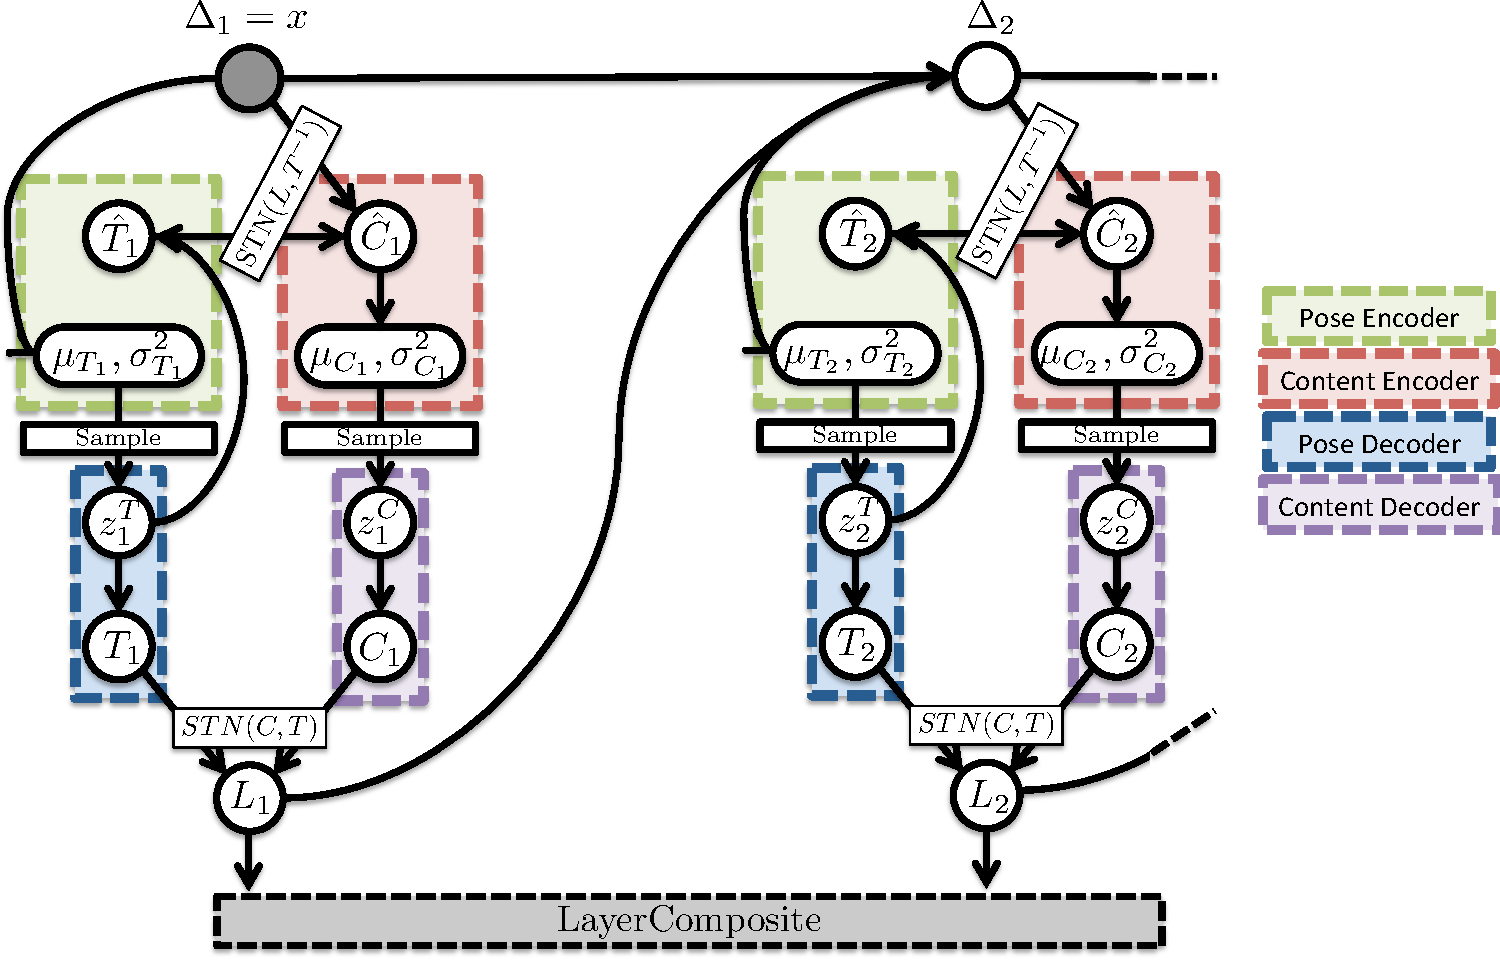
\includegraphics[width=0.65\linewidth]{figs/cstvae_diagram.pdf}\vspace{-3mm}
\end{center}
 \caption{\footnotesize
The CST-VAE network ``unrolled'' for two image layers.
 }
\label{fig:cstvae}
\end{figure}

%Intuitively the ST-VAE model should work well in factoring pose from content for images of single objects.
%However images generally contain multiple objects of different types with different poses --- we now present
%the Composited Spatially Transformed Variational Auto-encoder  (CST-VAE) model, which is able to factor
%the appearance of an image into the appearance of the different layers
%that create an image.  
%The CST-VAE model thus makes it possible to combine generative models for images
%of single objects to obtain a generative model of  images of multiple objects.  
%Among other things, the CST-VAE model allows us to tease
%apart the component layers (or objects) that make up an image and reason about occlusion.
%Furthermore, as we show in experiments, it can be trained in a fully unsupervised fashion using ordinary stochastic
%gradient descent methods.  %However we can also add labels or use semi supervised methods a la asdfasdf

%In the CST-VAE model, we  assume that images are generated by first independently generating a sequence of layers 
% via the ST-VAE model, then compositing layers from front to back to form a final observed image.  See Figure~\ref{fig:compositestvae_gm} for
% a graphical model depiction of the CST-VAE generative model and Figure~\ref{fig:cartoon}
% for a simplified cartoon illustration of the same process.  We assume that each layer is generated using the same ST-VAE model
% (i.e. parameters are shared across image layers). To composite these layers,  we use  the
%classic \emph{over operator} from computer graphics~\citep{porter1984compositing}.
%In the two-layer setting
%with only foreground and background layers, this over operator reduces to a simple $\alpha$-weighted
%convex combination of foreground and background pixels, but it extends in a natural (and differentiable)
%way to handle multiple layers. % associativity of the over operator

We now turn back to the multi-layer CST-VAE model, where again the task is to parameterize the recognition model $Q$. 
In particular we would like to 
avoid learning a model that must make a ``straight-shot'' joint prediction of all objects and their poses in an image.
Instead our approach is to perform inference over a single layer at a time from front to back, each time removing the contribution of a layer
from consideration until the last layer has been explained.


We proceed recursively: to perform inference for  layer $L_i$, we assume that the latent parameters $z^C_i$ and $z^T_i$ are responsible for explaining
some part of the residual image $\Delta_i$ --- i.e. the part of image that has not been explained by layers $L_1, \dots, L_{i-1}$ (note that $\Delta_1=x$).
We then use the ST-VAE module (both the decoder and encoder modules) 
to generate a reconstruction of the layer $L_i$ given $\Delta_i$.  Finally to compute the residual image to be explained by future layers, we set
$\Delta_{i+1} = \max (0, \Delta_i - L_i)$.  Assuming that observed and predicted pixel values are between 0 and 1, $\Delta_i-L_i$ can be negative, which breaks interpretability of the layers --- the ReLU transfer function, $ReLU(\cdot)=\max(0, \cdot)$, serves to ensure that the residual image can always itself be interpreted as an image.

Note that our encoder for layer $L_i$ requires that the decoder has been run for layer $L_{i-1}$.  Thus it's not possible to separate the generative
and recognition models into disjoint parts as in the ST-VAE model.  Figure~\ref{fig:cstvae} unrolls the entire CST-VAE network (combining
both generative and recognition models) for two layers.

















\section{Evaluation}

In all of our experiments we use the same training settings used in~\cite{Kingma2014}; that is,  
we use Adagrad for optimization with minibatches of 100  with a learning rate of 0.01
and a weight decay corresponding to a prior of $\mathcal{N}(0,1)$.
We initialize weights in our network using the heuristic of ~\cite{glorot2010understanding}.
However for the pose recognition modules in the ST-VAE model, we have found it useful to
specifically initialize biases so that poses are initially close to the identity transformation (see~\cite{jaderberg2015spatial}).

For all three models (VAE, ST-VAE, CST-VAE),
we experiment with between 10 and 50  dimensions for the latent variables $z$.
We parameterize content encoders and decoders
by using a two layer fully connected MLP with 256 dimensional
hidden layers and ReLU nonlinearities.
For pose decoders and encoders we also use two layer fully connected MLPs, but 
using 32 dimensional hidden layers and Tanh nonlinearities.\footnote{
%
We have found this choice of Tanh vs. ReLU makes a significant
difference in practice.
\kevin{Why?}
}
Finally for spatial transformer modules, we always resample onto a grid that is the same size as the original
image.


\Jon{For binary images, it is common to have a sigmoid at the end of the VAE decoder.
However we have found that it is often more numerically stable in these situations to first apple the spatial transformation, then
to apply the sigmoid after the transformation.
}

\subsection{Evaluating the Spatially transformed Variational Autoencoder alone}

We first evaluate our ST-VAE (single layer) model alone on the MNIST dataset~\citep{lecun1998gradient}
and a derived dataset, \emph{TranslatedMNIST}, in which we randomly translated each  $28\times 28$ MNIST example
within a $36\times 36$ black image.  In both cases, we binarize the images by thresholding at value 128.
Figure~\ref{fig:vae_stvae_learning_curves} plots train and test curves over 250000 gradient steps

Ordinary and Translated MNIST comparing
\begin{itemize}
\item ordinary vae
\item stvae model
\end{itemize}


\begin{itemize}
\item show pretty images
\item show that we often converge in first few iterations in pose and start to learn style after that
\end{itemize}



\Jon{Accuracy of classification of latent layer?}



\begin{figure}[t]
\begin{center}
\subfigure[]{
\raisebox{3mm}{
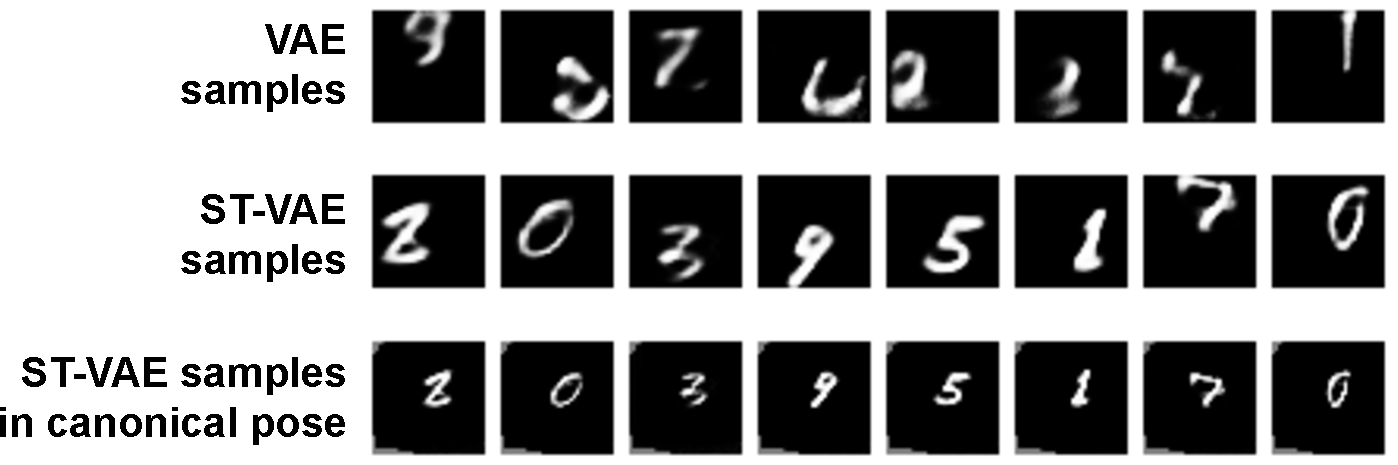
\includegraphics[width=0.45\linewidth]{figs/vae_stvae_samples.pdf}
\label{fig:vae_stvae_samples}
}
}
\qquad
\subfigure[]{
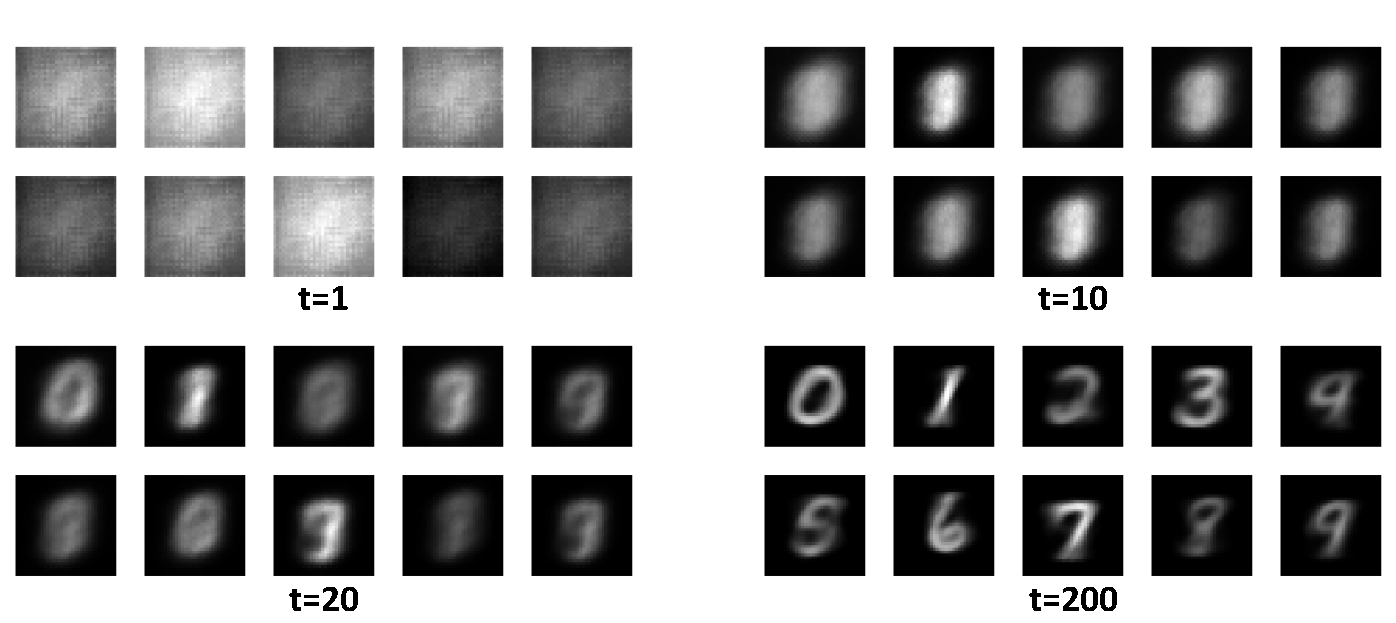
\includegraphics[width=0.45\linewidth]{figs/stvae_averageddigits.pdf}
\label{fig:stvae_averageddigits}
}
\end{center}
 \caption{
 \subref{fig:vae_stvae_samples} Comparison of samples from the VAE and ST-VAE generative models.  
 For the ST-VAE model, we show both the sample in its canonical pose and the final generated image.
  \subref{fig:stvae_averageddigits}  Averaged images from each MNIST class as learning progresses ---
  we typically see pose variables converge very quickly.
 }
\end{figure}

\begin{figure}[t]
\begin{center}
\subfigure[]{
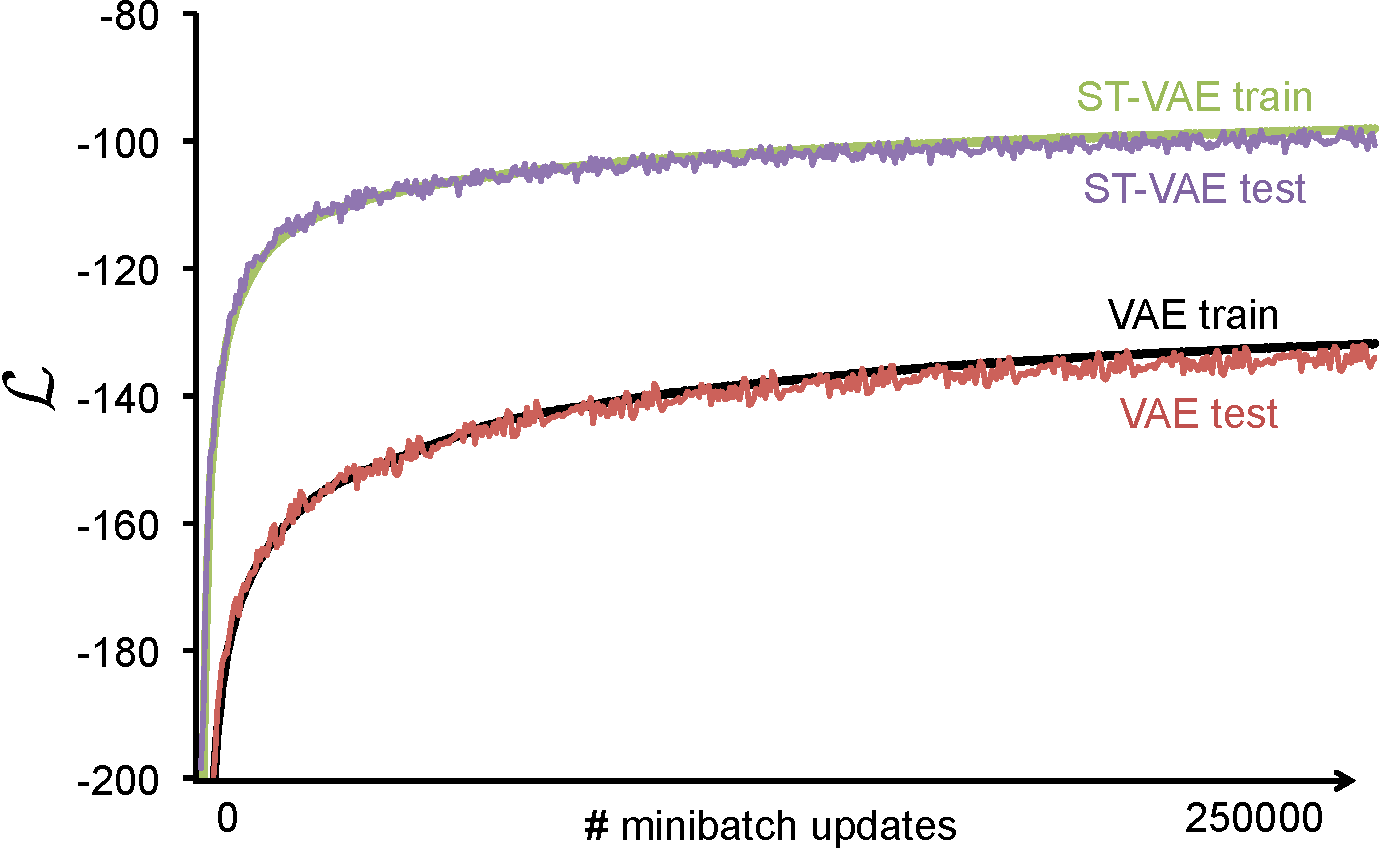
\includegraphics[width=0.30\linewidth]{figs/vae_stvae_learning_curves.pdf}
\label{fig:vae_stvae_learning_curves}
}
\subfigure[]{
\raisebox{12mm}{
\footnotesize
\begin{tabular}{lcc} 
\hline 
%\multicolumn{1}{r|}{Proposals} & \multicolumn{2}{c}{GT} & \multicolumn{2}{c}{multibox} \\
%\multicolumn{1}{r|}{Descriptions} & GEN & GT & GEN & GT \\
 & Train Accuracy & Test Accuracy \\
\hline 
\multicolumn{3}{l}{On translated (36x36) MNIST} \\
\hline
VAE + supervised & 0.771 & 0.146 \\
ST-VAE + supervised & 0.972 & 0.964  \\
directly supervised & 0.884 & 0.783 \\
Directly supervised with STN & 0.993 & 0.969  \\
\hline 
\multicolumn{3}{l}{On original (28x28) MNIST} \\
\hline 
Directly supervised & 0.999 & 0.96   \\
\hline
\end{tabular}%
}
\label{fig:vae_stvae_classification}
}
\end{center}

 \caption{
 \subref{fig:vae_stvae_learning_curves} Train and test (per-example) lower bounds on log-likelihood 
for the vanilla VAE and ST-VAE models on the Translated MNIST data;
 \subref{fig:vae_stvae_classification} Classification accuracy obtained by supervised training using latent encodings
 from VAE and ST-VAE models.  More details in text.
 }
\end{figure}









\subsection{Evaluating the CST Variational Autoencoder}

Dataset
\begin{itemize}
\item MNIST superimposed
\item Can we also get this to work with silhouettes of different grayscale levels?
\item CIFAR???
\item Textures
\end{itemize}


Explain encoder/decoder architectures for pose and style

Show reconstruction results on MNIST and samples from a single STAEVB module within the network



\begin{figure}[t]
\begin{center}
\subfigure[]{
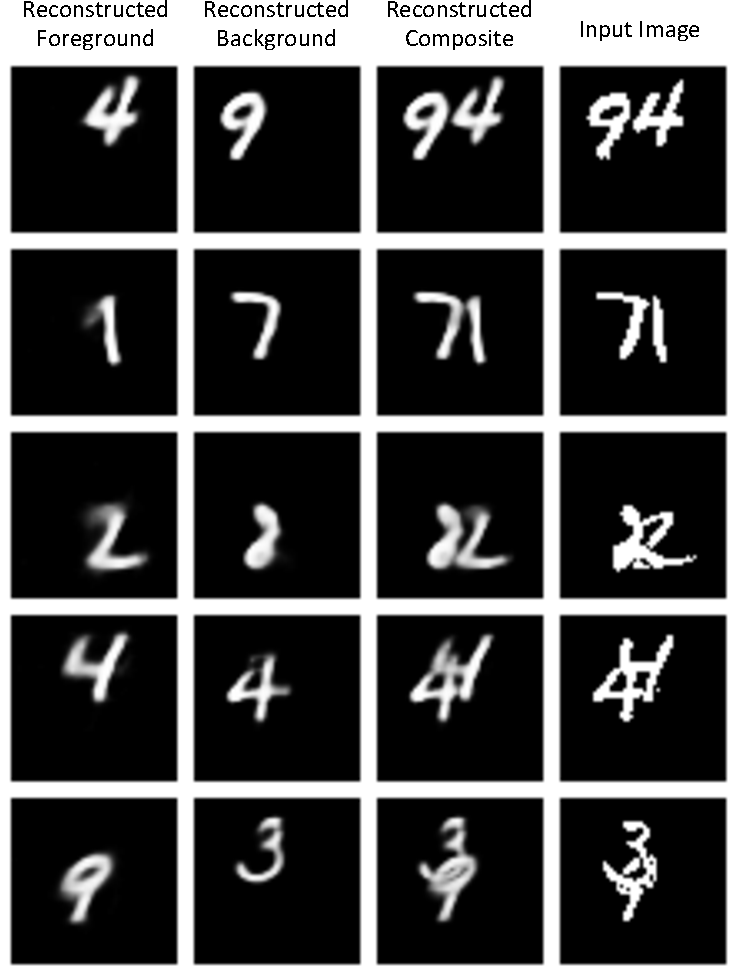
\includegraphics[width=0.4\linewidth]{figs/cstvae_reconstructions.pdf}
\label{fig:cstvae_reconstructions}
}\qquad\qquad
\subfigure[]{
\raisebox{5mm}{
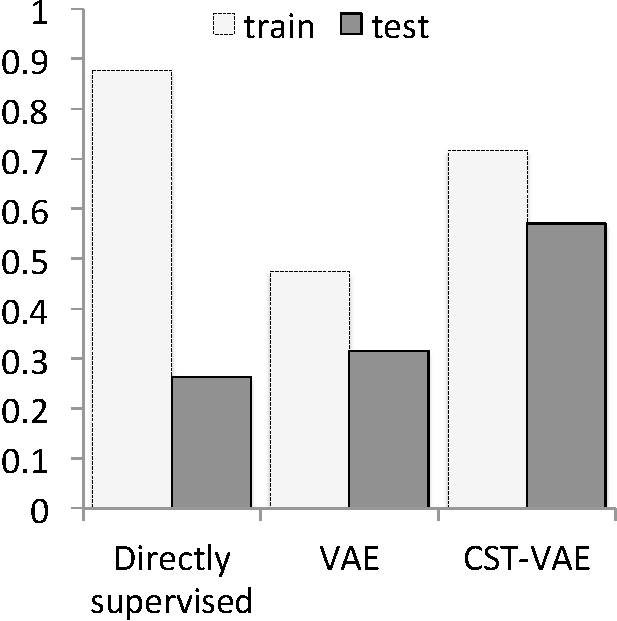
\includegraphics[width=0.3\linewidth]{figs/cstvae_classification.pdf}
\label{fig:cstvae_classification}
}
}
\end{center}
 \caption{
 \subref{fig:cstvae_reconstructions}  Images from the Superimposed MNIST dataset with visualizations of
 intermediate variables in the neural network corresponding to first and second layers and the final reconstruction;
 \subref{fig:cstvae_classification}
 Classification accuracy obtained by supervised training using latent encodings
 from VAE and CST-VAE models on the Supervised MNIST dataset.  More details in text.
 }
\end{figure}




\subsection{Partially observed data}




\subsection{Supervised training}
compare accuracy on something



\subsection{With Textures???}














\section{Conclusion}
\vspace{-2mm}

We have shown how to combine an old idea --- of interpretable, generative, layered models of images --- 
with modern techniques of deep learning, in order to tackle the challenging problem of intepreting images in the presence of occlusion in an entirely unsupervised fashion. We see this is as a crucial stepping stone to future work on deeper scene understanding, going beyond simple 
feedforward supervised prediction problems.
In the future, we would like to apply our approach to real images, and possibly video.
This will require extending our methods to use convolutional networks, and may
also require some weak supervision (e.g., in the form of observed object class labels associated with layers)
or curriculum learning to simplify the learning task.


\eat{
Probabilistic graphical models with generative semantics were popular in vision not too many years ago 
but in recent years have largely fallen out of favor. These more traditional generative models typically are burdened by slow inference and can be surprisingly unwieldy since good accuracy often relied on maintaining code for a large family of different handcrafted visual features which had to be tuned appropriately.  However our work suggests that we may not want to throw the baby out with the bathwater just yet.  
Probabilistic generative models often have interpretable  semantics  and allow us to learn with supervision, weak/semi-supervision and no supervision all within a unified framework.  Our models are examples of this type of interpretable generative model that \emph{can} coexist with rich feature hierarchies that are automatically tuned by end-to-end backpropagation. They are also fast at test time, requiring just a single forward pass through a neural network.  Finally they can be trained with no labeled data. Thus we believe that this combining of the best of both worlds will be a fruitful area of future work in both representation learning
and computer vision.
}

%\section*{Appendix}
%
\subsection*{Appendix: Notation}


\begin{tabular}{cc}
VAE & \\
ST-VAE & \\
CST-VAE & \\
$x$ & b \\
 $x_i$ & d \\
  $L_i$ & d \\
   $C_i$ & d \\
   $T_i$ & d \\
$z^C_i$ & d \\
$z^T_i$ & d \\
$f_C(\cdot; \theta_C)$ & d \\
$f_T(\cdot; \theta_T)$ & d \\
$f_enc(\cdot ;\phi)$ & d \\
$P(x | z^C, z^T; \theta)$ & d \\
$Q(z^C, z^T | x; \phi)$ & d 
\end{tabular}



\subsubsection*{Acknowledgments}
We are grateful to Sergio Guadarrama and Rahul Sukthankar for reading and providing feedback on 
a draft of this paper.

\bibliography{iclr2016_conference}
\bibliographystyle{iclr2016_conference}

\end{document}
